
\subsection{آزمون جهش و کاربردهای آن}
توسعه‌دهندگان و پژوهش‌گران حوزه‌ی نرم‌افزار علاقه مند به اندازه‌گیری موثر بودن مجموعه‌های آزمون می‌باشند. توسعه دهندگان به دنبال آن هستند که بدانند مجموعه آزمون‌های آنها می‌تواند به خوبی خطاها را تشخیص دهد و پژوهشگران به دنبال مقایسه‌ی روش‌های مختلف آزمون و اشکال زدایی\endnote{Debugging}  هستند. به طور ایده آل افراد تمایل دارند که بدانند تعداد خطاهایی که یک مجموعه آزمون می‌تواند شناسایی کند چه مقدار است اما از آنجا که خطاها ناشناخته هستند باید از اندازه‌گیری  وکالتی\endnote{Proxy Measurment} استفاده شود. یکی از اندازه‌‌‌گیری‌های شناخته شده امتیاز جهش \endnote{Mutation Score} می‌ باشد که توانایی مجموعه آزمون در تمیز دادن نسخه‌ی اصلی برنامه از تعداد زیادی نسخه‌های متفاوت را اندازه‌گیری می‌کند. این نسخه‌های متفاوت که تنها یک تفاوت کوچک نحوی نسبت به برنامه‌ی اصلی دارند جهش‌یافته\endnote{Mutant} نامیده می‌شوند. امتیاز جهش درصد جهش‌یافته‌هایی  است که توسط مجموعه آزمون از برنامه‌ی اصلی تمیز داده می‌شوند. به این صورت که این جهش‌یافته‌ها باعث شکست یک مورد آزمون می‌شوند در حالی که در نسخه‌ی اصلی مجموعه‌ی آزمون با موفقیت اجرا می‌گردد. جهش‌یافته‌ها با تزریق خطاهای ساختگی به برنامه‌ی تحت آزمون  ساخته می‌شوند.  نمونه‌ای از  جهش‌یافته‌ها  برای یک قطعه کد در شکل \ref{fig:mutant} آمده است. این خطاهای ساختگی با استفاده از عملگرهای جهش که از پیش تعریف شده‌اند ساخته می‌شود. نمونه‌ی این عملگرها جایگزینی عملگرهای ریاضی یا رابطه‌ای، تغییر شرط شاخه \endnote{Branch Condition} و یا حذف یک عبارت است\cite{just2014mutants}. تحلیل آزمون در موارد زیر کاربرد دارد:
\begin{itemize}
	\setlength\itemsep{.01em}	
	\item 
	ارزیابی مجموعه آزمون
	\item 
	انتخاب مجموعه آزمون
	\item 
	 کمینه سازی مجموعه آزمون
	\item 
	 تولید مجموعه آزمون
	\item 
	مکان‌یابی خطا
	\item 
	پیش‌بینی خطا
\end{itemize}

\begin{figure}[H]
	\centering
	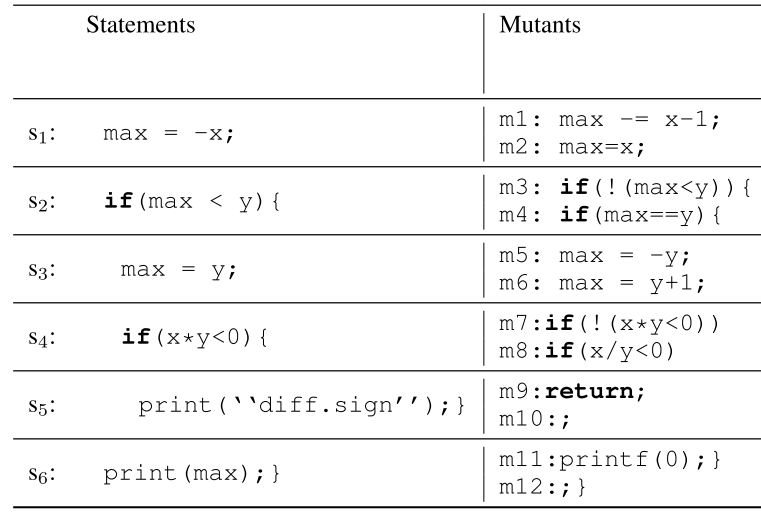
\includegraphics[width=.6\textwidth]{images/mutants.PNG}
	\caption{ نمونه‌ای از جهش‌یافته‌های یک برنامه \cite{moon2014ask}}
	\label{fig:mutant}
\end{figure}
جاست\LTRfootnote{Just} و همکاران در پژوهش خود به بررسی این موضوع پرداخته‌اند که آیا جهش‌یافته‌ها می‌توانند جایگزین مناسبی برای خطاهای واقعی باشند یا خیر\cite{just2014mutants}. در پژوهش‌های گذشته بررسی شده بود که میان جهش‌یافته‌های ساده و پیچیده وابستگی وجود دارد ولی وابستگی میان جهش‌یافته‌های ساده و خطاهای واقعی مشخص نیست. جاست و همکاران دو مجموعه‌ی آزمون برای هر خطا در نظر گرفتند که مجموعه‌ی اول در نسخه‌ی حاوی خطا با موفقیت گذرانده می‌شود. مجموعه‌ی دوم در نسخه‌ی حاوی خطا شکست می‌خورد و در نسخه‌ی رفع خطا با موفقیت اجرا می‌شود. نتایج نشان می‌دهد که مجموعه‌ی آزمون دوم دارای امتیاز جهش بالاتری می‌باشد که نشان می‌دهد هر خطا به یک جهش‌یافته وابستگی دارد. لازم به ذکر است که سعی شده که دو مجموعه‌ی آزمون دارای پوشش یکسانی باشند زیرا پوشش بیشتر می‌تواند امتیاز جهش بیشتر بیانجامد. همچنین مشخص شد که  
73 \lr{\%} 
خطاهای واقعی با جهش‌یافته‌هایی که  با عملگرهای متدوال تولید شده‌اند وابستگی دارند. در این پژوهش خطاهایی که با جهش‌یافته‌ها وابستگی ندارند در سه دسته قرار می‌گیرند : دسته اول نیازمند عملگرهای قوی تری هستند، دسته‌ی دوم نیازمند عملگرهای جدیدی هستند و دسته‌ی سوم با جهش‌یافته‌ها وابستگی ندارند.\\
\subsubsection{مکان‌یابی خطا}
روش‌هایی که از جهش‌یافته‌ها به منظور مکان‌یابی خطا استفاده می‌کنند دارای شباهت‌هایی با روش‌های پیش‌بینی خطا هستند. در هر دوی این روش‌ها از معیارهایی  کد منبع استفاده می‌شود تا احتمال وجود خطا محاسبه شود. دو تفاوت عمده‌ی این دو حوزه این است که اولا در مکان‌یابی خطا از روش‌های یادگیری ماشین استفاده‌ی چندانی نمی‌شود، ثانیا در مکان‌یابی خطا وجود خطا به وسیله شکست مورد آزمون یا گزارش خطا محرز شده است. با توجه به شباهت‌های موجود میان این دو حوزه در ادامه چند مقاله که با استفاده از آزمون جهش به مکان‌یابی خطا پرداخته‌اند را بررسی می‌کنیم. \\

موون\LTRfootnote{Moon} و همکاران در مقاله‌ی خود بر اساس دو فرض روشی به منظور مکان‌یابی خطا ارائه داده‌اند. فرض اول بیان می‌کند که  در یک برنامه‌ی حاوی خطا جهش و یا اصلاح یک عبارت خطا دار نسبت به جهش یک عبارت درست می‌تواند موارد آزمون بیشتری را  با موفقیت بگذراند. فرض دوم  بیان می‌کند که جهش عبارات صحیح نسبت به جهش یک عبارت غلط موجب می‌شود موارد آزمون بیشتری شکست بخورند. بر اساس این دو فرض معیاری به نام "مشکوک بودن" \endnote{Suspiciousness} ارائه گردیده است که دو فرض را فرموله می‌کند. این معیار بر اساس تعداد شکست و موفقیت موارد آزمون در نسخه‌ی اصلی و جهش‌یافته عمل می‌کند. سپس با رتبه بندی عبارات بر اساس این معیار عبارت حاوی خطا مشخص می‌گردد. در این پژوهش روش جدیدی نیز به منظور ارزیابی روش پیشنهادی ارائه شده است که برخی از مشکلات روش پیشین را بر طرف نموده است. در نهایت روش مکان‌یابی ارائه شده با دو روش ارزیابی شده و نتایج نشان می‌دهد فرضیات پژوهش درست بوده‌اند \cite{moon2014ask}. \\

پاپاداکیس  و تراوون \LTRfootnote{Papadakis and Traon} در مقاله‌ی خود به این نکته اشاره کرده‌اند  که استفاده از تحلیل جهش در گذشته به دلیل پر هزینه بودن چندان مورد توجه قرار نمی‌گرفته است اما امروزه با وجود ابزارهای مقیاس پذیر، نمونه گیری و انتخاب جهش می‌توان به خوبی از تحلیل جهش در انجام پژوهش‌های مختلف استفاده کرد\cite{papadakis2015metallaxis}. آنها روشی را برای مکان‌یابی خطا بر اساس دو مشاهده ارائه کرده‌اند. در مشاهده‌ی اول دیده می‌شود که خطای موجود در یک عبارت رفتار مشابهی با جهش در همان عبارت نشان می‌دهد. در مشاهده‌ی دیگر دیده می‌شود که اگر  خطا و جهش در دو عبارت متفاوت باشند رفتار متفاوتی خواهند داشت. منظور از رفتار مشابه موفقیت یا شکست در یک آزمون است. بر اساس این دو مشاهده معیاری برای مشکوک بودن عبارات تعیین می‌گردد. این پژوهش بیان می‌کند که مناسب بودن موارد آزمون تاثیر مستقیمی بر عملکرد روش مکان‌یابی خطا  دارد. همچنین یک مجموعه‌ی کوچک از جهش‌یافته‌ها می‌تواند به اندازه‌ی مجموعه‌ای کامل تاثیر گذار باشد. \\

\subsubsection{مدل‌های یادگیری و جهش‌یافته‌ها}
 
 هااو\LTRfootnote{Hao} و همکاران با ارایه‌ی مجموعه‌ای از معیارها و استفاده از یادگیری ماشین مدلی را ارائه داده‌اند که به وسیله‌ی آن بتوان تشخیص داد علت شکست در آزمون رگرسیون وجود خطا است یا منسوخ \endnote{Obsolete} شدن یک مورد آزمون\cite{hao2013bug}. هفت معیار ارائه شده در این پژوهش مرتبط با گراف فراخوانی، تغییر در فایل‌ها و تعداد شکست در آزمون‌ها بوده است.  هااو و همکاران به منظور به دست آوردن مجموعه داده‌ی حاوی خطا، به صورت دستی بر اساس استانداردهایی  از پیش تعریف شده خطاهایی را در کد قرار داده‌اند. بدین منظور عباراتی به صورت تصادفی که در سراسر کد محصول قرار دارند انتخاب شدند و به وسیله‌ی عملگرهای جهش خطاهایی تولید شده است. به منظور بدست آوردن آزمون‌های منسوخ شده، مجموعه آزمون‌هایی از نسخه‌ی قبلی برنامه بر روی کد  نسخه‌ی بعدی بکار گرفته شده است. سپس با استفاده از روش ارزیابی میان دسته‌ای\endnote{Cross-validation} به آموزش و آزمایش مدل ساخته شده پرداخته می‌شود. نتایج پژوهش نشان می‌دهد که روش پیشنهادی زمانی که بر روی یک نسخه‌یا نسخه‌های مختلف از یک برنامه اعمال شود نتایج خوبی دارد (80\lr{\%} دقت) اما زمانی که بر روی برنامه‌های مختلف اعمال شود ( مجموعه آموزش از یک برنامه و آزمون بر روی برنامه‌ای دیگر) موثر نیست. نتایج نشان می‌دهد تکنیک‌ها مکان‌یابی خطا نتیجه‌ی مثبتی بر تشخیص نوع خطا که مربوط به محصول است یا آزمون، ندارد.\\
 
 بوئز\LTRfootnote{Bowes} و همکاران معیارهایی را مبتنی بر جهش معرفی کردند و  از ترکیب آنها با معیارهای سنتی و شئ گرایی، یک مدل پیش‌بینی ساخته شده است\cite{bowes2016mutation}. 8 عملگر جهش در نظر گرفته شده و برای هر یک از آنها یک معیار ایستا (بدون اجرای کد) و چهار معیار پویا ساخته شده و در مجموع 40 معیار جهش ارائه شده است. به این دلیل میان معیار ایستا و پویا تمایز قائل شده‌اند که اگر معیارهای ایستا به تنهایی  پیش‌بینی را بهبود بخشند بدون نیاز به موارد آزمون می‌توان از آنها استفاده کرد، در واقع دامنه‌ی کاربرد روش گسترده‌تر می‌گردد. نتایج پژوهش نشان می‌دهد که استفاده از معیارهای جهش بهبود قابل توجهی را در پیش‌بینی خطا به وجود می‌آورد. همچنین معیارهای پویا و ایستا در کنار یکدیگر توانایی پیش‌بینی مناسبی دارند ولی استفاده‌ی جداگانه از آنها تاثیر چندان مثبتی نخواهد داشت. این پژوهش از دو جنبه حائز اهمیت می‌باشد. یکی اینکه اولین پژوهش در زمینه‌ی پیش‌بینی خطاست که از تحلیل جهش استفاده کرده است. دوم آنکه مشابه ترین پژوهش به پژوهش کنونی می‌باشد. 
 
 
 
 
 
 
 
 
 
 
 
 
 
 
 
 
 
 
 
 
 

